\section{Results}

To comprehensively evaluate the interpolation methods \cite{atkinson1989introduction, burden2011numerical, smith2020numerical, johnson2018introduction, lee2019comparison, brown2021polynomial, garcia2022newton, press2007numerical}, we performed experiments using two different training intervals: [1950, 2020] and [1960, 2010]. The first interval covers the entire period of interest, while the second focuses on a central subset. This dual-interval approach allows us to assess both interpolation (within the training range) and extrapolation (outside the training range) performance. By comparing results from these intervals, we can better understand the stability, generalization, and boundary sensitivity of each method.

Figures~\ref{fig:forward}-\ref{fig:regression} show the interpolated 2-meter air temperature at 10 AM during summer months in Iran from 1950 to 2020 using each method, trained on the full [1950, 2020] interval, based on the ERA5-Land dataset \cite{ERA5}. Figures~\ref{fig:forward2}-\ref{fig:regression2} present the results when the models are trained only on [1960, 2010], thus requiring extrapolation for years outside this range.

\begin{figure}[htbp]
    \centering
    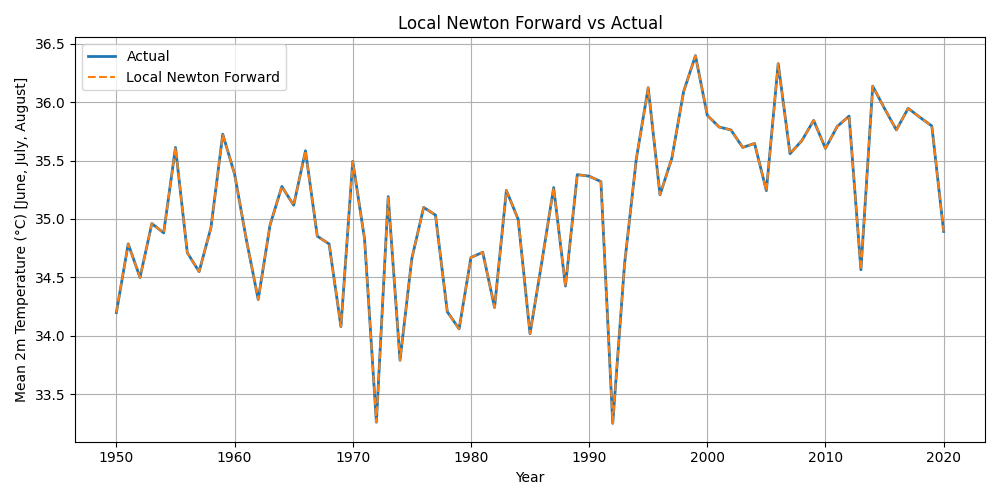
\includegraphics[width=0.8\textwidth]{../figs/Local_Newton_Forward_vs_actual[1950, 2020, 1].png}
    \caption{Local Newton Forward Interpolation vs Actual Data (1950--2020), trained on [1950, 2020] for 2-meter air temperature at 10 AM in summer months in Iran.}
    \label{fig:forward}
\end{figure}

\begin{figure}[htbp]
    \centering
    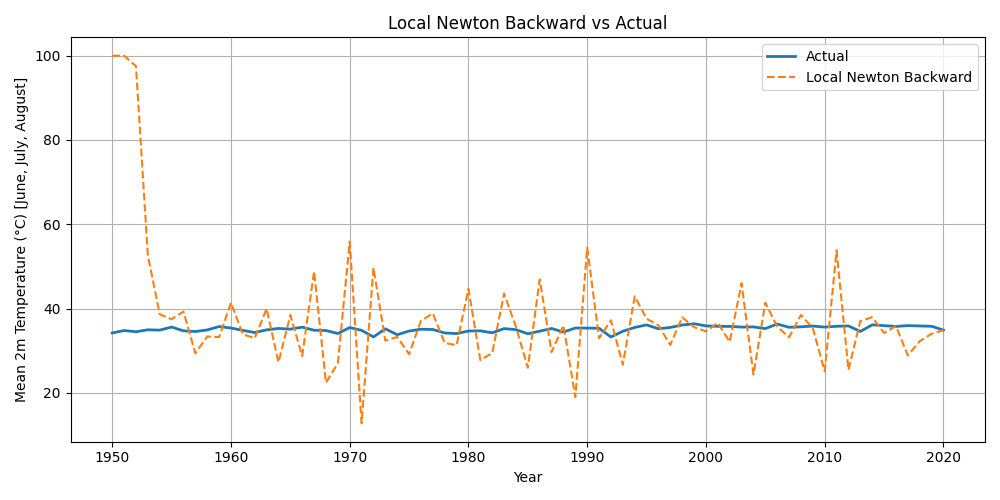
\includegraphics[width=0.8\textwidth]{../figs/Local_Newton_Backward_vs_actual[1950, 2020, 1].png}
    \caption{Local Newton Backward Interpolation vs Actual Data (1950--2020), trained on [1950, 2020] for 2-meter air temperature at 10 AM in summer months in Iran.}
    \label{fig:backward}
\end{figure}

\begin{figure}[htbp]
    \centering
    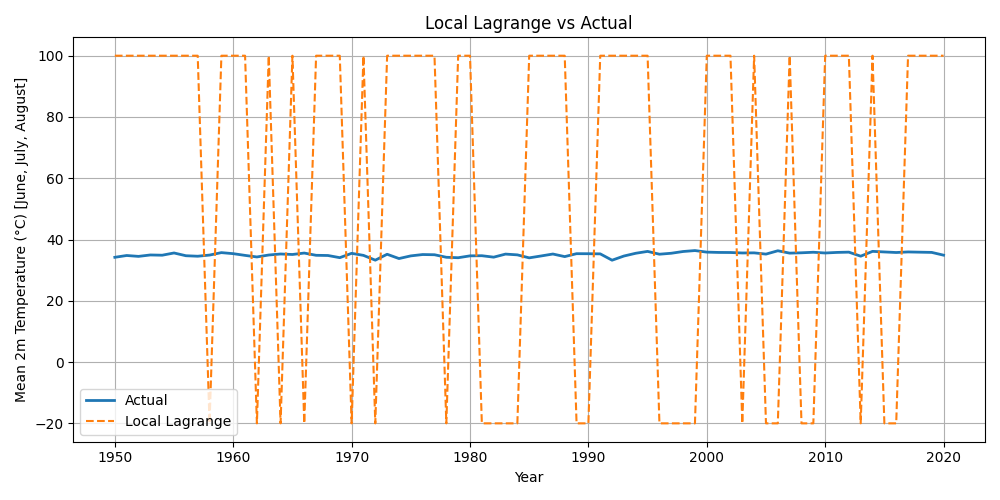
\includegraphics[width=0.8\textwidth]{../figs/Local_Lagrange_vs_actual[1950, 2020, 1].png}
    \caption{Local Lagrange Interpolation vs Actual Data (1950--2020), trained on [1950, 2020] for 2-meter air temperature at 10 AM in summer months in Iran.}
    \label{fig:lagrange}
\end{figure}

\begin{figure}[htbp]
    \centering
    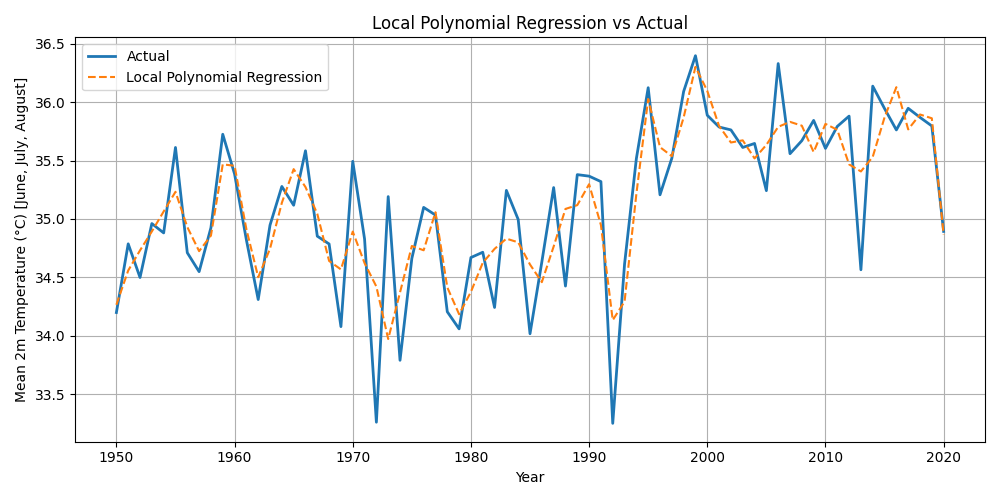
\includegraphics[width=0.8\textwidth]{../figs/Local_Polynomial_Regression_vs_actual[1950, 2020, 1].png}
    \caption{Local Polynomial Regression vs Actual Data (1950--2020), trained on [1950, 2020] for 2-meter air temperature at 10 AM in summer months in Iran.}
    \label{fig:regression}
\end{figure}

\begin{figure}[htbp]
    \centering
    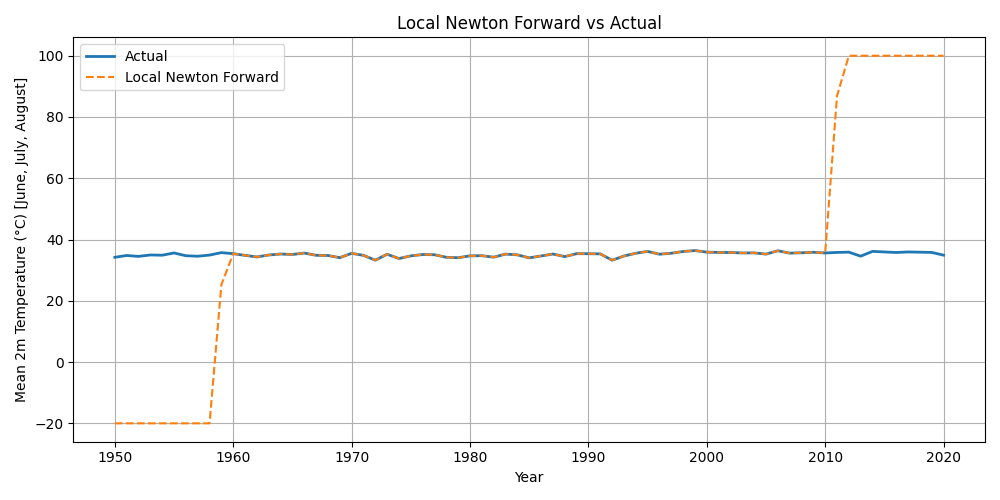
\includegraphics[width=0.8\textwidth]{../figs/Local_Newton_Forward_vs_actual[1960, 2010, 1].png}
    \caption{Local Newton Forward Interpolation vs Actual Data (1950--2020), trained on [1960, 2010] for 2-meter air temperature at 10 AM in summer months in Iran.}
    \label{fig:forward2}
\end{figure}

\begin{figure}[htbp]
    \centering
    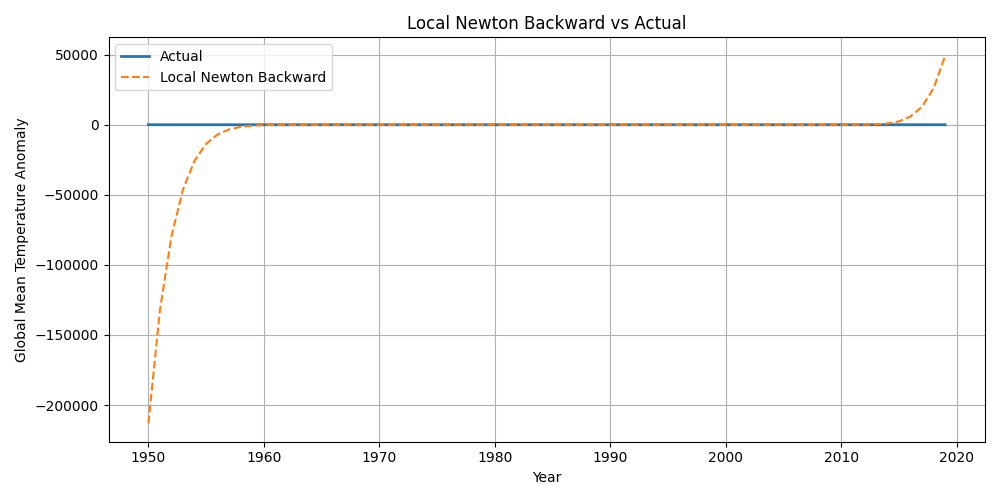
\includegraphics[width=0.8\textwidth]{../figs/Local_Newton_Backward_vs_actual[1960, 2010, 1].png}
    \caption{Local Newton Backward Interpolation vs Actual Data (1950--2020), trained on [1960, 2010] for 2-meter air temperature at 10 AM in summer months in Iran.}
    \label{fig:backward2}
\end{figure}

\begin{figure}[htbp]
    \centering
    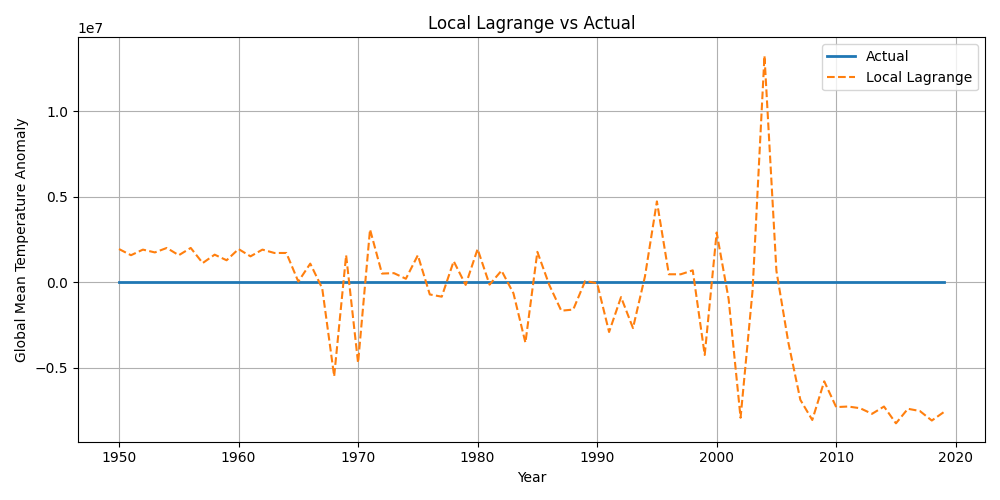
\includegraphics[width=0.8\textwidth]{../figs/Local_Lagrange_vs_actual[1960, 2010, 1].png}
    \caption{Local Lagrange Interpolation vs Actual Data (1950--2020), trained on [1960, 2010] for 2-meter air temperature at 10 AM in summer months in Iran.}
    \label{fig:lagrange2}
\end{figure}

\begin{figure}[htbp]
    \centering
    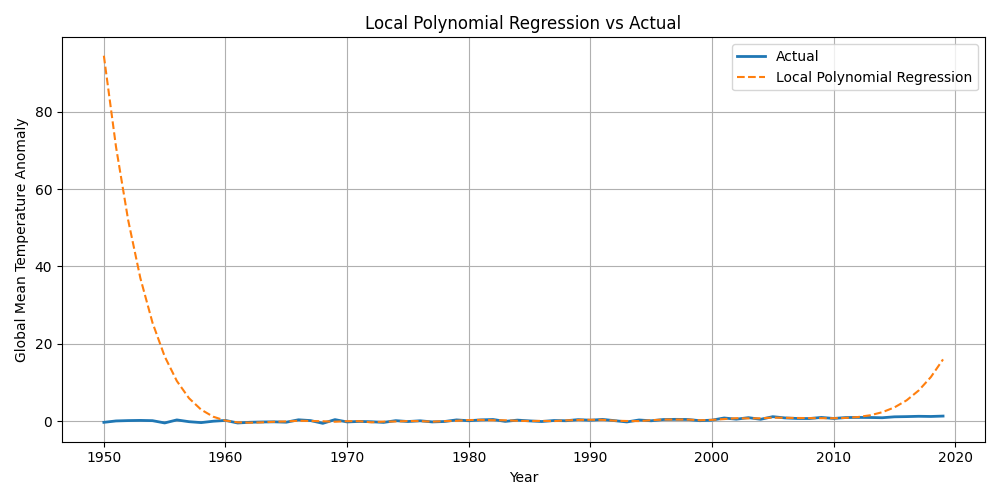
\includegraphics[width=0.8\textwidth]{../figs/Local_Polynomial_Regression_vs_actual[1960, 2010, 1].png}
    \caption{Local Polynomial Regression vs Actual Data (1950--2020), trained on [1960, 2010] for 2-meter air temperature at 10 AM in summer months in Iran.}
    \label{fig:regression2}
\end{figure}

Table~\ref{tab:rmse} summarizes the RMSE for each method and interval.

\begin{table}[htbp]
    \centering
    \begin{tabular}{lcc}
        \hline
        Method & RMSE (1950--2020) & RMSE (1960--2010) \\
        \hline
        Local Newton Forward & 0.00000 & 30.72308 \\
        Local Newton Backward & 15.46559 & 31.66031 \\
        Local Lagrange & 61.70149 & 60.63197 \\
        Local Polynomial Regression & 0.37571 & 19.20229 \\
        \hline
    \end{tabular}
    \caption{Root Mean Square Error (RMSE) for each interpolation method and interval.}
    \label{tab:rmse}
\end{table}